
%! TEX root = paper.tex

\section{Results}
\label{sec:results}

The descrived methods have been tested in a desktop scene covering an area of 7x3 meters. The path taken to acquire training and testing data covering the mentioned area can be seen in~\ref{fig:large_desktop_train_test}. The dataset contains 84 frames for training and 69 for testing.\\

\begin{figure}[htpb]
  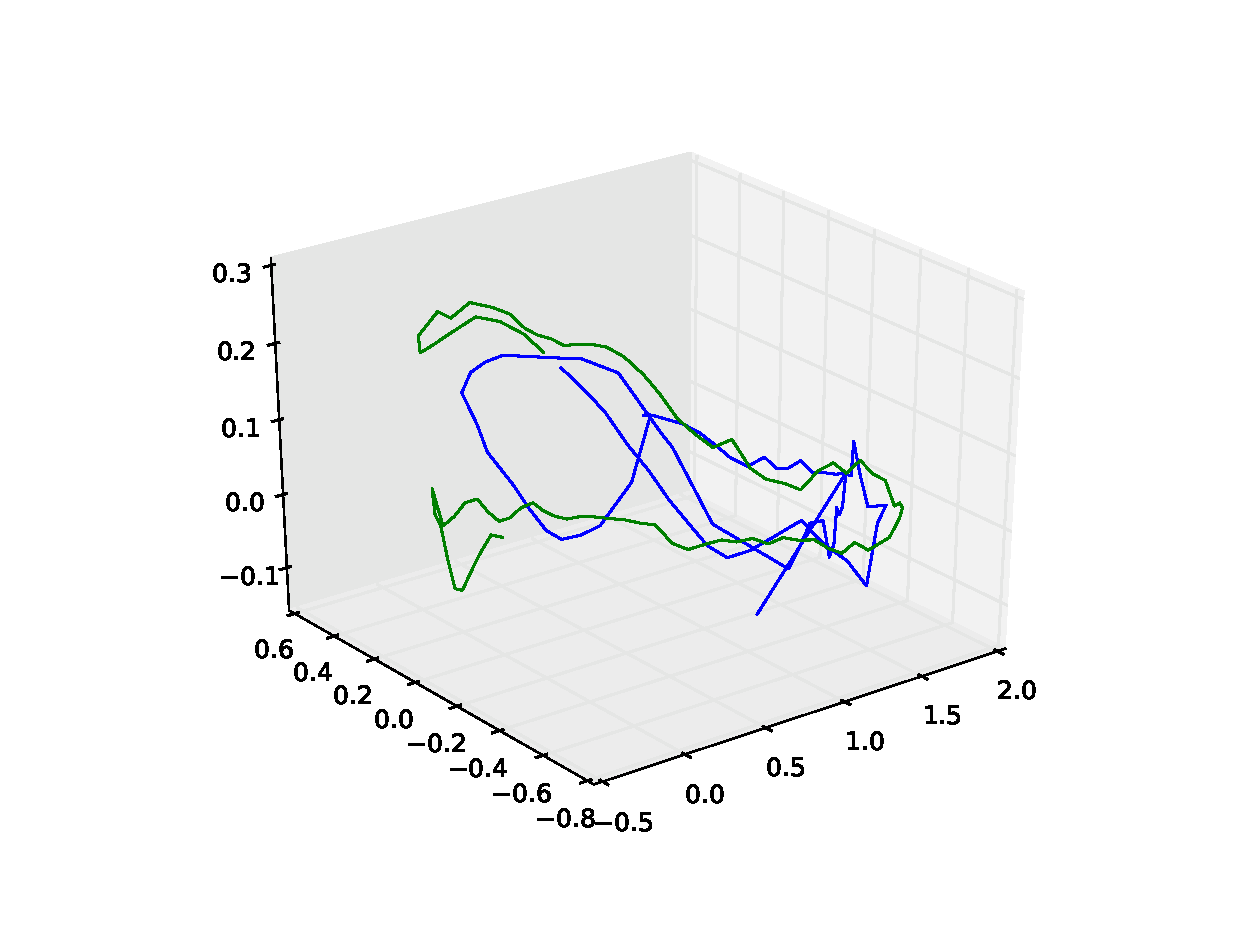
\includegraphics[width=\linewidth]{img/large_desktop/test_train_path.eps}
  \caption{In green, the path used for training. In blue, the path used for testing}
  \label{fig:large_desktop_train_test}
\end{figure}

\subsection{Multi Relocalizer}
\label{sub:multi_relocalizer_large}


\subsubsection{Extended Second-order Minimization \textit{Real Pose Finder}}
\label{ssub:extended_second_orther_minimization_real_pose_finder}

The performance of ESM Real Pose Finder is not great in this dataset as seen in~\ref{fig:desktop_2_CC_3pt_dist_1} although it was able to correctly relocalize in other datasets.\\

\begin{figure}[htpb]
  \includegraphics[width=1\linewidth]{img/large_desktop/CC_esm_dist.eps}
  \caption{Translation error histogram using CC \textit{Place Finder} and ESM \textit{Real Pose Finder}}
  \label{fig:desktop_2_CC_esm_dist_1}
\end{figure}


\subsubsection{Three-point \textit{Real Pose Finder}}
\label{ssub:large_three_point_real_pose_finder}

On the other side, the Three-point \textit{Real Pose Finder} works very well as seen in~\ref{fig:desktop_2_CC_3pt_dist_1}. It can correctly retrieving the pose of 42 of the 69 frames. This method is very dependent on the results of the \textit{Place Finder}, and on this dataset, the cross correlation method was not very effective. Better results on it would help iprove the results of this method and the ESM method.\\

\begin{figure}[htpb]
          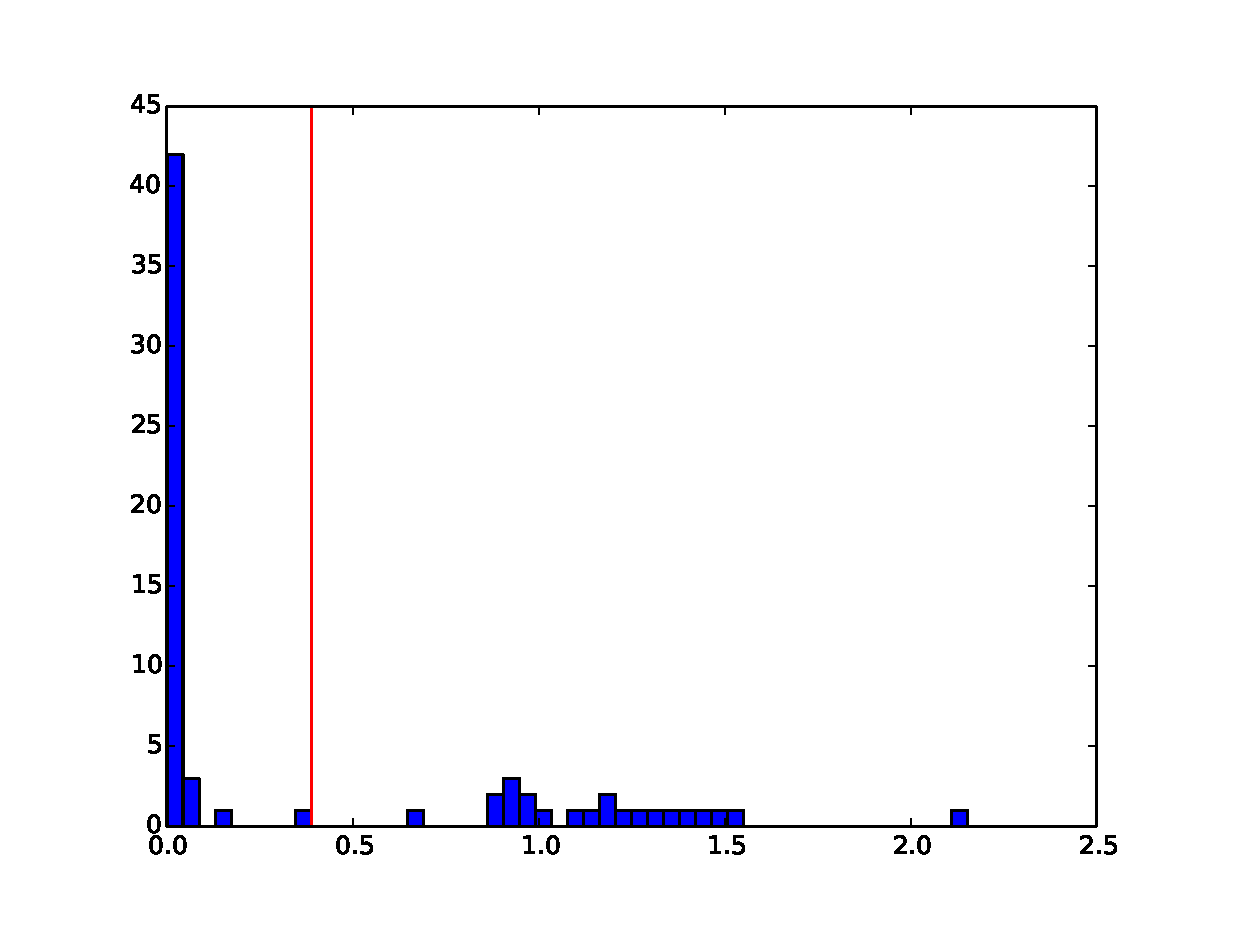
\includegraphics[width=1\linewidth]{img/large_desktop/CC_3pt_dist.eps}
          \caption{Translation error histogram using CC and P3P, with the mean marked as a red line}                
          \label{fig:desktop_2_CC_3pt_dist_1}
\end{figure}


\subsection{Ferns}
\label{sub:large_ferns}

Finally, as an alternative to the PTAM relocalization method, it was proposed to use machine learning techniques, more concretely \textit{ferns}. In~\cite{Ozuysal2010} it is shown that \textit{ferns} can be used to distinguish up to around 200 different classes. We applied the method to this dataset where there are 1730 classes. In figure~\ref{fig:large_desktop_ferns_dist} it can be seen that almost 50 of the 69 frames where correctly relocalized. Which is more than using Multi Relocalizer with the three-point \textit{Real Pose Finder}. The classifier was trained with 100 \textit{ferns} of 12 tests each.\\

It should be noticed that not all points need to be well classified, as long as more than 3 points are correctly identified then the posterior RANSAC will find and use the once that agree.\\

The three-point with CC method and this one, can correctly relocalize the same number of frames. Probably there is one part of the dataset that is more ambiguous and difficult to recognize and both algorithms struggle with it.\\

\begin{figure}[htpb]
          \includegraphics[width=1\linewidth]{img/large_desktop/ferns_100_dist.eps}
          \caption{Translation error histogram using \textit{ferns} with 12 tests, with the mean marked as a red line}                
          \label{fig:large_desktop_ferns_dist}
\end{figure}

\section{Execution time}
\label{sec:execution_time}

In figure~\ref{fig:exec_time} the mean execution time of relocalization is shown. There, it can be seen that the ESM and the P3P methods are the faster while the method using \textit{ferns} classifier is slower and is sensitive to the number of classes. Also, while ESM and P3P use optimized third party libraries, the \textit{ferns} based classifier has been integrally implemented by us, maybe not achieving the best performance. The used training time for the classifier can be seen in figure~\ref{fig:training_time}.\\

\begin{figure}[htpb]
  \centering
  \begin{bchart}[steps={0.2,0.4,0.6,0.8,1},max=1, scale=0.6]
  \bcbar[label= CC and ESM]{0.0437}
  \bcbar[label=CC and P3P]{0.0647}
  \bcbar[label=ferns 237 classes]{0.128}
  \bcbar[label=ferns 1730 classes]{0.933}
  \end{bchart}
  \caption{Single relocalization execution time}
  \label{fig:exec_time}
\end{figure}


\begin{figure}[htpb]
  \centering
  \begin{bchart}[step=10, max=70, scale=0.6]
    \bcbar[label=\quad 237 classes]{5.57}
    \bcbar[label=1730 classes]{63.11}
  \end{bchart}
  \caption{\textit{ferns} classifier training time}
  \label{fig:training_time}
\end{figure}
